\documentclass[10pt,conference,compsocconf]{IEEEtran}

\usepackage{hyperref}
\usepackage{graphicx}	% For figure environment
\usepackage{subfigure}
\usepackage{titling} % Customizing the title section
\usepackage{dblfloatfix}    % To enable figures at the bottom of page
\usepackage{kantlipsum}     % for random text

\begin{document}
\pretitle{\begin{center}\Huge\bfseries} % Article title formatting
\posttitle{\end{center}} % Article title closing formatting
\title{Road Segmentation challenge}

\author{
	% Your name
	\textsc{Niccol\`{o} Sacchi \& Valentin Nigolian} \& Theo Deprelle \\
	\normalsize{} \\
	% Your supervisors
	\textsc{Group:}
	\normalsize{RoadSegmentationFault}\\
	% Your institution
	\normalsize \'{E}cole polytechnique f\'{e}d\'{e}rale de Lausanne
}

\maketitle

\begin{abstract}
  The goal of this project is to segment satellite images in order to discriminate the roads from the background. Several approaches have been tried in the past, most of them required a lot of preprocessing and did not gained great performances. Invented in the late 20th century, the convolutional neural networks (CNNs) only recently were successfully applied to images classification and segmentation problems and performed considerably better than other techniques.
  The model we used in this project consists of a CNN whose input can be an image of any size and the output is the respective mask of roads (ground-truth). Our model makes use of on-the-fly data augmentation, Dropout layers, LeakyReLU activation functions to reduce overfitting and improve the training. Moreover, we adopted two simple but effective techniques to improve the predictions. We will also show that, according to our tests, our model outperforms the considered baselines.
\end{abstract}

\section{Introduction}
The segmentation problem can be defined as the problem of assigning a class label to a set of pixels so to classify part(s) of an image.
The goal of this project is to segment the roads in satellite images so to extract the mask of the roads. The metric used to evaluate the prediction of the roads is the F1 score that combines the precision, i.e. the fraction of correctly predicted roads among all the predicted roads, and the recall, i.e. the fraction of correctly predicted roads among all the true roads. The formula of the F1 score is the following:
$$F1=2\frac{pr}{p+r}$$ $$\textrm{where} \quad p=\frac{TP}{TP+FP} \textrm{,} \quad r=\frac{TP}{TP+FN}$$

Only in recent years, thanks the increase in computing performance and the possibility to exploit GPUs to parallelize computation, CNNs were able outperform most of the techniques in solving different tasks, e.g. image classification, image segmentation, natural language processing, handwriting generation, automatic game playing and many others. The strengths of the CNNs derives from a hierarchy of filters which are learnt during the training phase. Thanks to these filters, the CNNs are capable of producing more and more complex features, i.e. high level representation of the input, as the image goes deeper in the network. However, a drawback of CNNs is the need of a large, fully-labeled dataset. This drawback can be compensated with data augmentation.
In the following sections we will give an overview of the techniques we tried focusing in particular to the CNN we implemented and tuned. Section~\ref{sec:data-analysis} gives an overview of the dataset, Section~\ref{sec:models-methods} proposes some approaches to the problem and explains the design of the cnn we used, Section~\ref{sec:results} shows and demonstrate the results reached with the explained model, Section~\ref{sec:furture-work} proposes some next steps that could be undertook to further improve the model.

\begin{figure}
	\centering
	\begin{minipage}{0.2\textwidth}
		\centering
		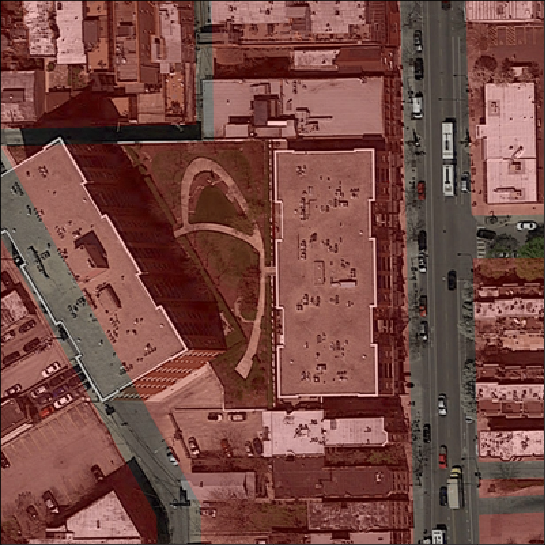
\includegraphics[width=1\textwidth]{img/building.png}
	\end{minipage}
	\begin{minipage}{0.2\textwidth}
		\centering
		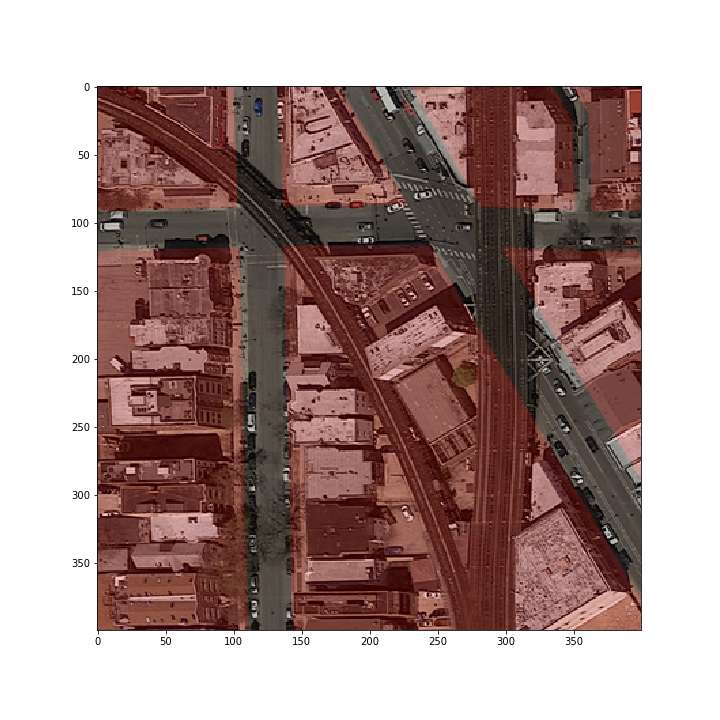
\includegraphics[width=1\textwidth]{img/highway.png}
	\end{minipage}
	\begin{minipage}{0.2\textwidth}
		\centering
		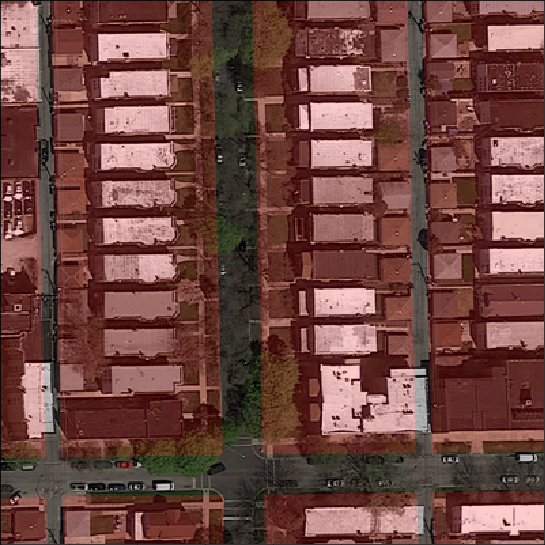
\includegraphics[width=1\textwidth]{img/trees.png}
	\end{minipage}
	\begin{minipage}{0.2\textwidth}
		\centering
		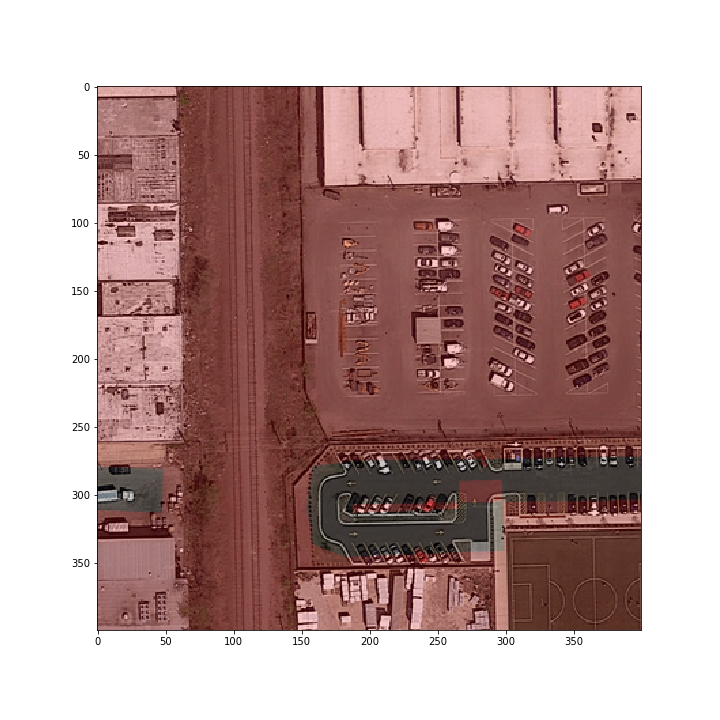
\includegraphics[width=1\textwidth]{img/parkinglot.png}
	\end{minipage}
	\caption{Corner cases in which roads are covered by (a) buildings, (b) railroads, (d) trees and also show the ambiguity of parking lots in (e)}
	\label{fig:corner-cases}
\end{figure}
%\begin{figure}
%	\centering
%	\begin{minipage}[b]{.4\textwidth}
%		\centering
%		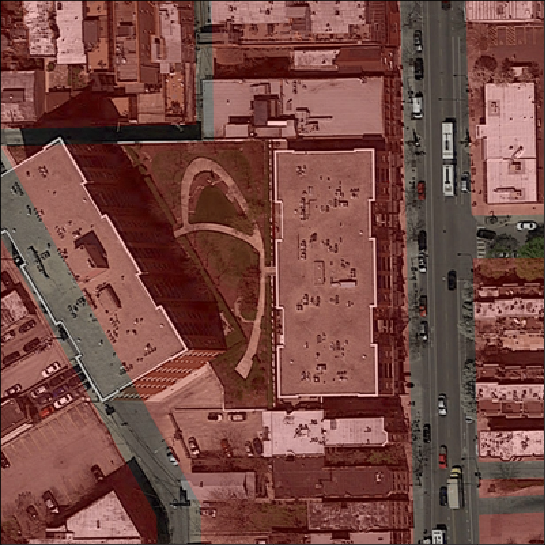
\includegraphics[width=.4\textwidth]{img/building.png}\quad
%		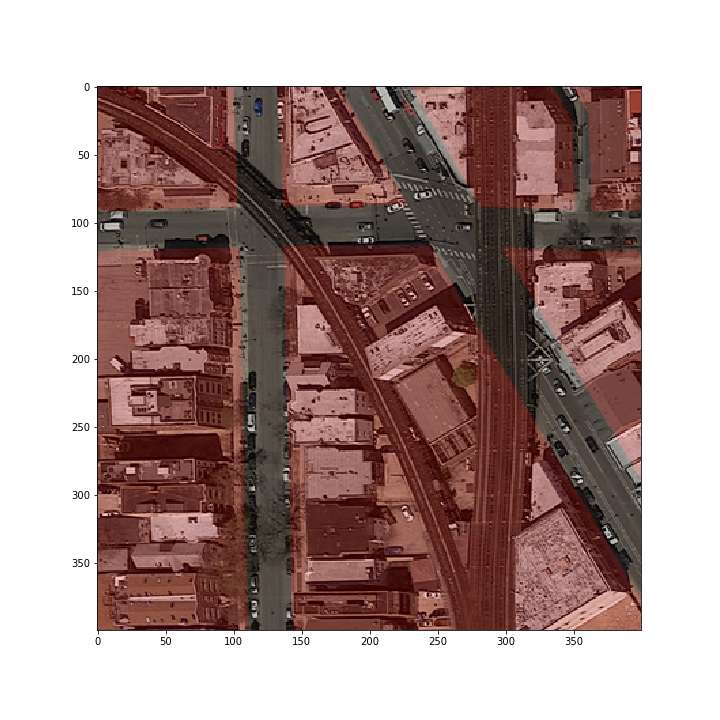
\includegraphics[width=.4\textwidth]{img/highway.png}\quad
%		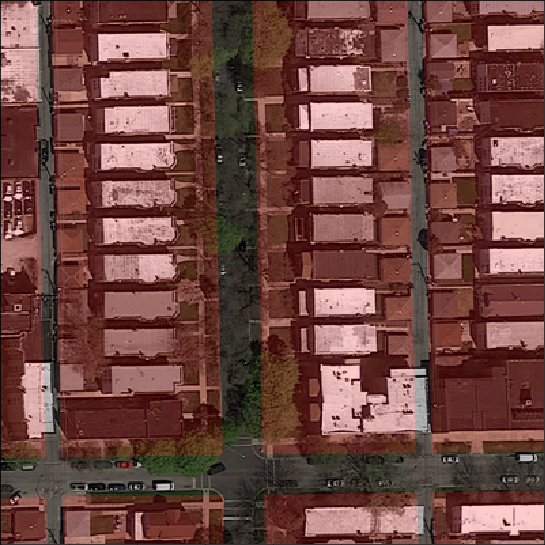
\includegraphics[width=.4\textwidth]{img/trees.png}\quad
%		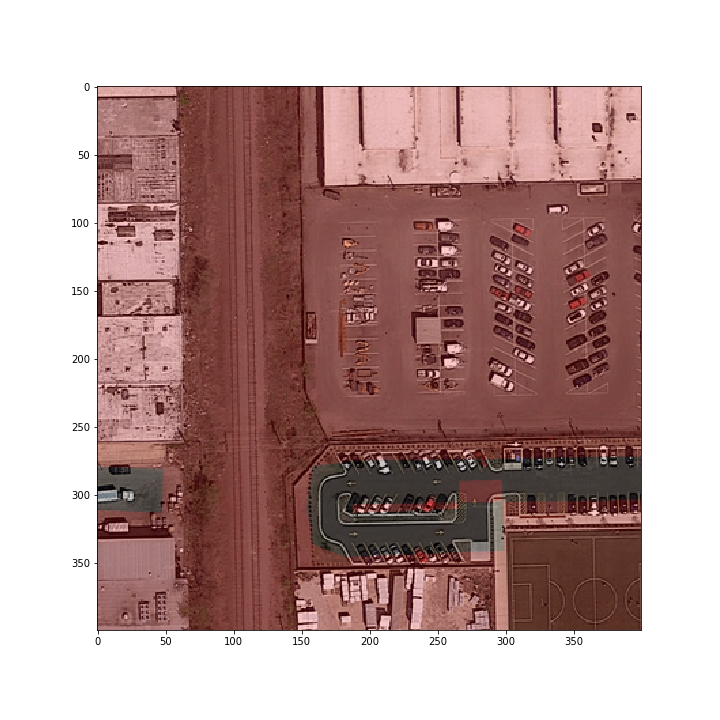
\includegraphics[width=.4\textwidth]{img/parkinglot.png}
%		\caption{Corner cases in which roads are covered by (a) buildings, (b) highways, (d) trees and also show the ambiguity of parking lots in (e)}\label{label-b}
%	\end{minipage}
%\end{figure}

%\begin{figure}[!ht]
%	\centering
%	\subfloat[][]{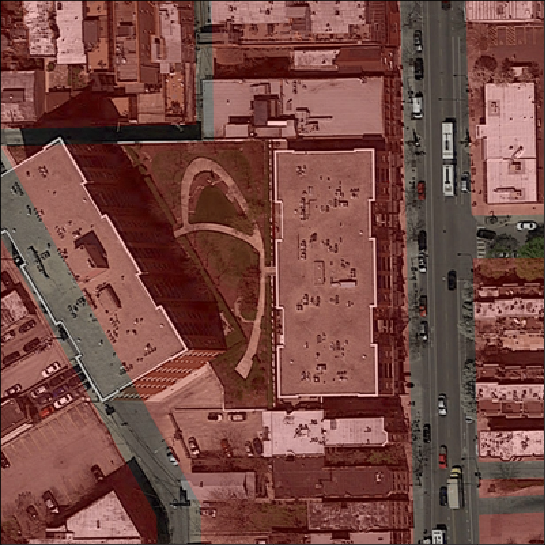
\includegraphics[width=.4\textwidth]{img/building.png}}\quad
%	\subfloat[][]{\includegraphics[width=.4\textwidth]{}}\\
%	\subfloat[][]{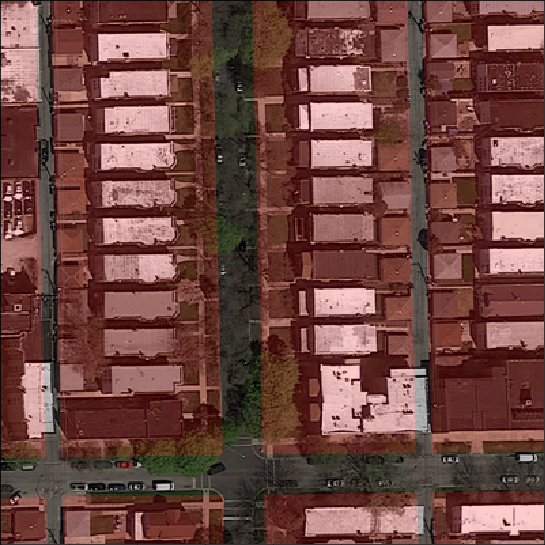
\includegraphics[width=.4\textwidth]{img/trees.png}}\quad
%	\subfloat[][]{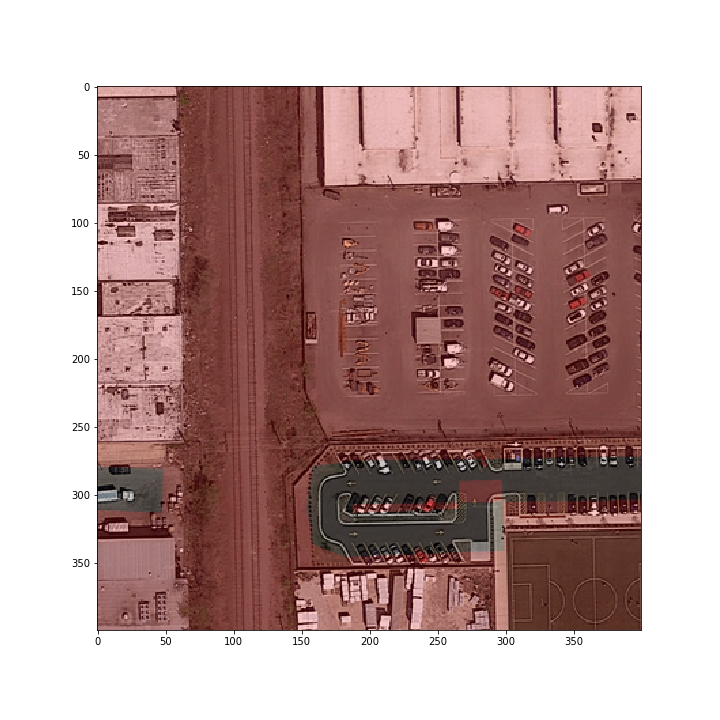
\includegraphics[width=.4\textwidth]{img/parkinglot.png}}
%	\caption{Corner cases in which roads are covered by (a) buildings, (b) highways, (d) trees and also show the ambiguity of parking lots in (e)}
%	\label{fig:sub1}
%\end{figure}

\section{Exploratory data analysis}
\label{sec:data-analysis}
We are given two sets of images acquired from GoogleMaps: (1) a train set composed by RGB images of size $400*400$ pixels and the respective ground-truth images, i.e. images of the same size where white pixels represent roads and black pixels represent the background, (2) a test set composed by RGB images $608*608$ pixels whose ground-truth has to be produced.
The aim of the project is to label patches of $16*16$ pixels, therefore, depending on the methodology used, pixels of the provided ground-truth may have to be grouped and averaged so to provide the class label for that patch. We adopted a threshold of $0.25$, if the average of the pixels in a patch was above the threshold then that patch was labeled as road, otherwise it was labeled as background.
By taking a look at the train set and its masks we could notice the problem had its non-trivialities, e.g. ambiguity of parking lots, roofs of the same color of the roads and trees, shadows, buildings, railroads and cars covering the surface of the roads, Figure \ref{fig:corner-cases}. Those problems can be solved only if we consider also the neighborhood of each patch to correctly classify it. That task can be achieved with feature extraction, either manually, with complex and advanced techniques, or automatically by a CNN.

\section{Models and Methods}
\label{sec:models-methods}
The first techniques we studied involved feature extraction using interesting, still complex and not very efficient techniques that fails in more extreme cases, e.g. when there are object obstructing the view of the road or there is a change of brightness through different images. Such techniques involved for example computation of the gradient at each pixel (so to exploit the fact that roads have continuity in one direction, i.e. a gradient {\raise.17ex\hbox{$\scriptstyle\sim$}}0), the use of an edge detection algorithm to extract the boundaries of the objects and the use of vector graphics to represent images with geometrical primitives such as points, lines, curves, and shapes or polygons~\cite{HORMESE20161460}. Given the complexity of those solutions and poorness of the results when compared to the CNNs, we opted for the latter which are well know for the little preprocessing needed and great efficiency in solving these kind of tasks.
We started from three very simple baselines: (1) a model that predicts all as road (notice that, since the metric chosen is the F1 score computed on the road predictions, a model that predicts all as background would have higher accuracy but an F1 score of zero), (2-3) we considered each $16*16$ patch as an input and for each one of them we produced 6 simple features extracted from the mean and the standard deviation of each RGB channel in the patch. The obtained dataset has been used to train a logistic regression and a random forest. The F1 scores of these three baselines is shown in Figure \ref{fig:baselines}. As expected, this analysis shows that those methods fails in this complex task if more advanced features extraction is not in place.
Therefore, we started searching and studying solutions based on CNNs. We found two main approaches: (1) design a CNN which segment the input image and outputs directly the mask for the roads~\cite{lis2016}, (2) reduce the segmentation problem to a classification problem, i.e. build a CNN that given as input a single patch, possibly with a bigger context (neighborhood of that patch), labels that patch as either road or background~\cite{dario2016}. We tried both the techniques but then opted and focused on (1) since it required almost no preprocessing and showed better results.
\begin{figure}[tbp]
	\centering
	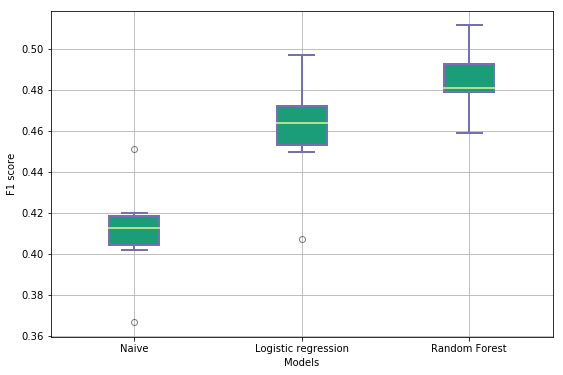
\includegraphics[width=0.8\columnwidth]{img/boxplots_naive.png}
	\caption{Distribution of the F1 scores computed on a 6-fold cross validation on the three considered baselines.}
	\vspace{-3mm}
	\label{fig:baselines}
\end{figure}

\subsection{CNN design}
\begin{figure}[tbp]
	\centering
	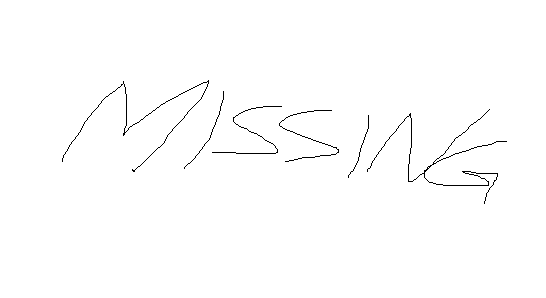
\includegraphics[width=0.8\columnwidth]{img/missing.png}
	\caption{Scheme of the final model used to obtain an F1 score of ... }
	\vspace{-3mm}
	\label{fig:cnn-model}
\end{figure}
\begin{figure}[tbp]
	\centering
	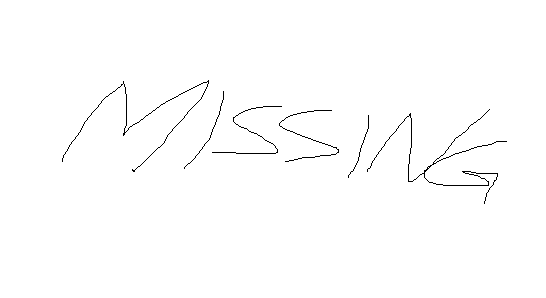
\includegraphics[width=0.8\columnwidth]{img/missing.png}
	\caption{Activations of the first convolutional layer: with ReLU on the left and with Leaky ReLU on the right. As can be noticed the number of dead filter decreased sensibly meaning the model was learning more reasonable features.}
	\vspace{-3mm}
	\label{fig:dead-filters}
\end{figure}

\subsection{Our CNN model}
Given the differences in size between train images and test images, we decided to build a CNN which could take as input an image of any size and output the estimated probability of being a road for each patch of that image. To achieve such a CNN we did not used any dense layer, since it requires an input of fixed size, and designed it such that it reduced each side of the input image by a factor equal to the width of the patch we wanted to predict so to obtain an output mask of size $H/n*W/n$ where n is the width of the patch. We tried both predicting $8*8$ patch-wise and $16*16$ patch-wise and observed better results when predicting $8*8$ patch-wise. The structure of our CNN is depicted in Figure \ref{fig:cnn-model}. Since we experienced problems of GPU memory filling, we could only adopt convolutional layers of higher number of filters after reducing the size of the input image, i.e. the first layers have bigger inputs and less filters while the last layers have smaller inputs but can have more filters \footnote{The output of a convolutional layer, when strides is $1*1$ and padding is used, is $H * W * \#filters$ where $H*W$ is the size of the input.}.

The most common activation function used after convolutional layer is the ReLU. However, since we have experienced the problem of dead filters \footnote{Dead filters are filters that always output zero for any input. This may happen when, during training, the weights are updated in such a way that the neuron will never activate on any input again which lead to a gradient of zero and no update of the weights.}, we have switched to the Leaky ReLU, i.e. a variant of the ReLU which has a small positive gradient for negative inputs:
$$f(x)=max(\alpha x, x)$$
Where $\alpha$ is the slope for negative inputs and is usually a small value ${\raise.17ex\hbox{$\scriptstyle\sim$}}0.01$.
This choice solved the problem of dead filters as can be seen in Figure \ref{fig:dead-filters}.

We used $k$ max pooling layers with a pool size of $2*2$ where $2\textsuperscript{k}$ is the size of the patch we wanted to predict, e.g. to predict $8*8$ patch-wise we adopted 3 max pooling layers so to reduce the size of the input image by a factor of 8 on each side. Note that increasing the strides of the convolutional layer would lead to the same size reduction but we opted for max pooling so to automatically select the higher activations.

Moreover, after each max pooling layer we added a dropout layer, i.e. a regularization technique used to prevent overfitting by randomly setting to 0 a fraction of the input during the training phase. We have set the dropping rate for all the dropout layers to $0.25$.

\subsection{Data augmentation}
CNNs need a big training set in order to recognize the patterns proper of the roads otherwise it could overfit and just memorize the training images. Increasing the training set is a must and could greatly increase the performance of the model while reducing overfitting. Our model builds the batches of images on-the-fly applying rotation and/or mirroring to the original image. While each image of the batch is mirrored with a probability of $0.5$ we decided not to rotate each image by a random degree since most of the images, both in the test set and train set, have vertical and horizontal roads and we wanted our model to master the recognition of those roads. Rotation is done in the following way: an image of the batch is rotated by any degree with a probability of $0.2$ while is rotated by $90^\circ*k$ where $k=1,2,3,4$ with a probability of $0.8$. Figure \ref{fig:data-augmentation} shows an examples of data augmentation applied on an image. This data augmentation proved to be effective and our model learnt not only to recognize horizontal and vertical roads but also diagonal roads.
\begin{figure}[tbp]
	\centering
	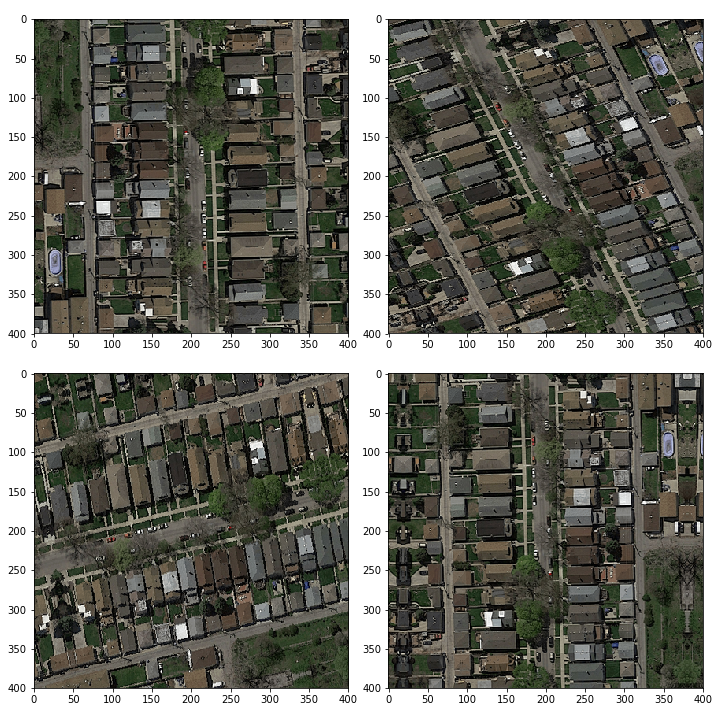
\includegraphics[width=0.8\columnwidth]{img/data_augmentation.png}
	\caption{At the top-left the original image, the other are example of augmentation of that image. After rotating the image, the points outside the boundaries are filled by reflecting the image so to always obtain an image of the same size ($400*400$).}
	\vspace{-3mm}
	\label{fig:data-augmentation}
\end{figure}

\subsection{Post-processing}
Once the model have been trained, its the predictions can be further improved in order to increase the F1 score. However, even if roads have some intuitive properties, e.g. starting from a road you can always reach the border the image, it is not trivial to improve a predicted mask of roads such that those properties are fulfilled. Therefore, we opted for two easier solutions that proved to increase the F1 score by a couple of percentage points.
\begin{itemize}
	\item We compute on the on the train images and its predictions the optimal threshold so that each patch whose probability is beyond that threshold is labeled as road. This step is simply done with a grid search and retrieving the threshold which corresponds to the maximum F1 score. This estimated optimal threshold will be used on the predictions of the test set to label each patch.
	\item To obtain the predictions of a test image, we mirror it and/or rotate it by $90^\circ*k$ where $k=1,2,3,4$ so to obtain 8 different predictions. Those predictions are then averaged to obtain the final prediction.
\end{itemize}

%~\cite{schwab00,wavelab,gentleman05}
%\begin{figure}[tbp]
%  \centering
%  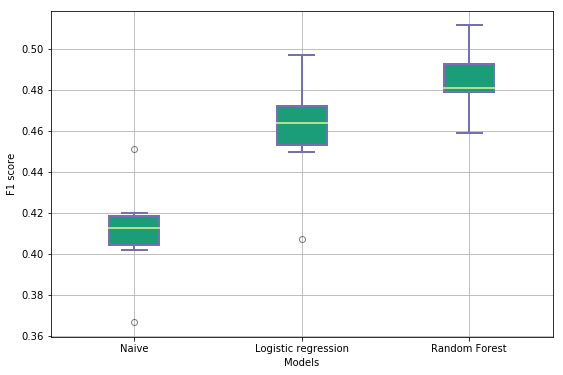
\includegraphics[width=\columnwidth]{img/boxplots_naive.png}
%  \caption{Signal compression and denoising using the Fourier basis.}
%  \vspace{-3mm}
%  \label{fig:denoise-fourier}
%\end{figure}
%
%\begin{enumerate}
%\item
%\end{enumerate}
%
%~\ref{tab:fourier-wavelet}.
%\begin{table*}[htbp]
%  \centering
%  \begin{tabular}[c]{|l||l|l|l|}
%    \hline
%    Basis&Support&Suitable signals&Unsuitable signals\\
%    \hline
%    Fourier&global&sine like&localized\\
%    wavelet&local&localized&sine like\\
%    \hline
%  \end{tabular}
%  \caption{Characteristics of Fourier and wavelet basis.}
%  \label{tab:fourier-wavelet}
%\end{table*}
%
%\footnote{For those who are
%  particularly interested, other common structures can be found at
%  \url{http://en.wikipedia.org/wiki/README} and
%  \url{http://www.gnu.org/software/womb/gnits/}.}.
%
%\texttt{.jpg} or
%
%\begin{equation}
%  \label{eq:linear}
%  y = mx + c
%\end{equation}
%(Equation~(\ref{eq:linear})).

\clearpage
\section{Theo's contribution}

\subsection{The data set}

The data set of aerial image the road detection have some inconsistency. Finding a process that will perform well is therefore quite challenging.

The first is the number of outlier that shares too few characteristic with the rest of the dataset images. Those are images of highways (3\% of the the dataset) and sea sides (2\% of the dataset) where the width and the shapes of the road and the background different from the rest of the set.
\begin{figure}[h]
  \centering
  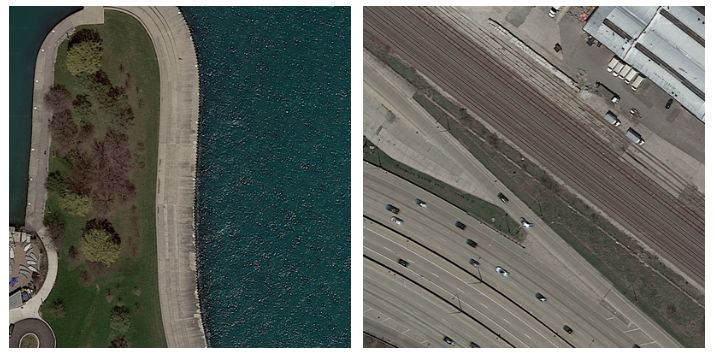
\includegraphics[width=\columnwidth]{img/outlayers.png}
  \caption{Outlayer of the dataset}
  \vspace{-3mm}
  \label{fig:outlayers}
\end{figure}

Since no sea side is present in the validation set we didn’t train on those images. One highway image was present in the validation set thought. To improve the result we are giving more highway images to the network by duplicating existing ones.

The second inconsistency is the labeling. In the following example you can see that the parking is not considered has a road despite the fact that it’s sharing all the aspect (color, cars on it, and texture of a road). We will see that our method actually learn to detect them despite the lack of annotations. That shows how close those elements are from actual roads. A better annotation should give us better results.

\begin{figure}
  \centering
  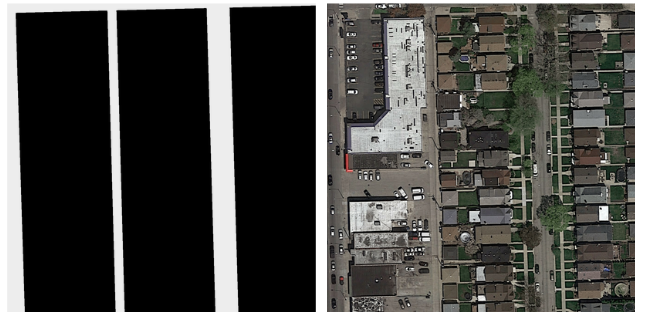
\includegraphics[width=\columnwidth]{img/wrongannots.png}
  \caption{Unlabeled road in the images}
  \vspace{-3mm}
  \label{fig:unlabeled}
\end{figure}

\clearpage

\subsection{The network}

\begin{figure}[h]
  \centering
  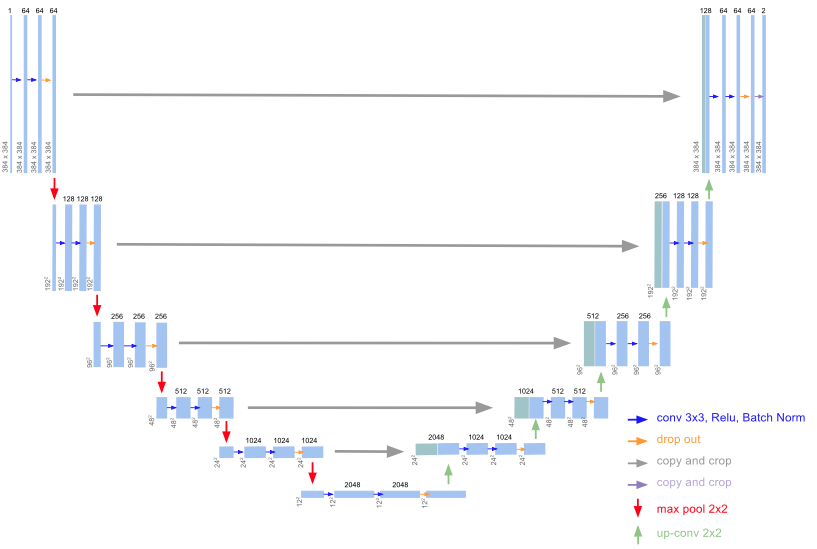
\includegraphics[width=0.95\columnwidth]{img/unet.png}
  \caption{UNet architecture}
  \label{fig:unet}
\end{figure}

The second experience we have tried is using the network UNet. This network was made to be used for medical image segmentation. Since our problem is close to what this network was made UNet was an ideal candidate.\\

U-Net network architecture is illustrated in \ref{unet} . It consists of a downsampling path (left side) and an upsampling path (right side). Boths share an architecture of a convolutional network. It consists of the repeated application of two 3x3 convolutions each followed by a rectified linear unit (ReLU) and a 2x2 max pooling operation with stride 2 for downsampling. We are using in total 28 differents convolution layers.\\

We added to the existing architecture a batch normalisation layer after every ReLU layers, a dropout layer before every max pooling and a fifth maxpooling operation.\\

We are using four skip connections that performs a concatenation with the output of the up-convolution and the input of the maxpooling.

The energy function is computed by a pixel-wise soft-max $S$ over the final feature map combined with the cross entropy loss function $E$.

\begin{equation}
	S(x) = \frac{exp(a_1(x))}{exp(a_1(x))+exp(a_0(x))}
\end{equation}

\begin{equation}
	E = \sum\limits_{x \in \Omega} w(x).log(S(x))
\end{equation}

Where $a_k(x)$ denotes the activation in feature channel $k$ at the pixel position $x$ of the image $\Omega$.

The input labels can either be 0 (background) 1 (road segment) or 2 (ignore part). The pixels labels 2 are ignore in the loss calculs and therefore have no impact on the training process.
\subsection{Data augmentation}

\begin{figure}[h]
 \centering
 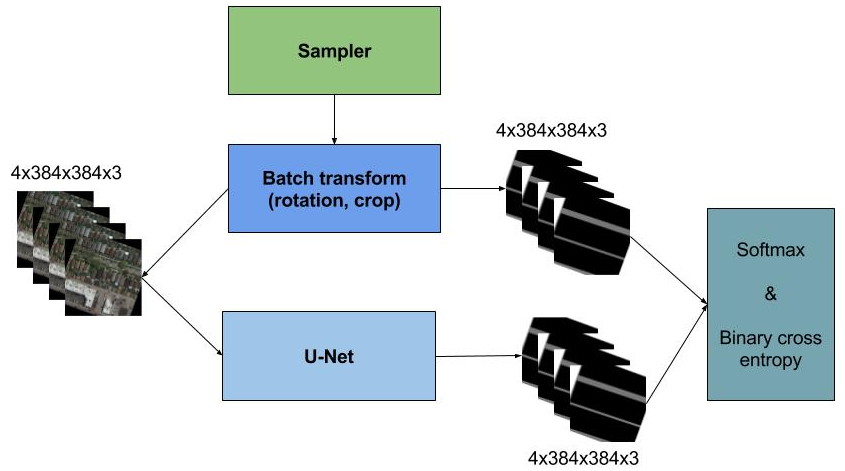
\includegraphics[width=0.7\columnwidth]{img/dataaug.png}
 \caption{Training step diagram.}
 \vspace{-3mm}
 \label{fig:denoise-fourier}
\end{figure}

We trained the network of patch of 384x384 selected randomly in the image. We selected a batch of 4 images every iteration to train the network.\\

Using this method our result were good but it appears that diagonals part of the roads were not detected correctly therefore some modification were needed.

This was because the majority of the images of the training set didn’t had diagonal lines.\\

To correct this problem we randomly rotate the batch after every training step. This allows us to have a better diagonal detection because we were feeding every kind of road orientation to the network.

\begin{figure}[h]
 \centering
 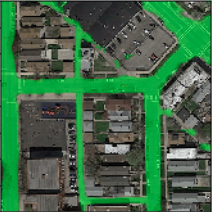
\includegraphics[width=0.35\columnwidth]{img/diagonals.png}
 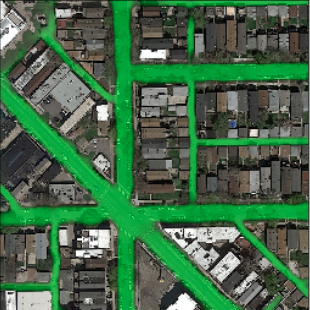
\includegraphics[width=0.35\columnwidth]{img/diagonals_corrected.png}
 \caption{On the left we can see that the diagonals are not detected well. On the contrary, on the right, when we are randomly rotating the images all the diagonals are well detected}
 \vspace{-3mm}
 \label{fig:diagonal}
\end{figure}

The sides of the rotated image needed to be treated carefully. Before backpropagating the loss we are setting the loss of the sides pixels to 0. This was made by assigning the label 2 (ignore pixel) to the ground-thrush image after the rotation.\\



\begin{figure}[h]
 \centering
 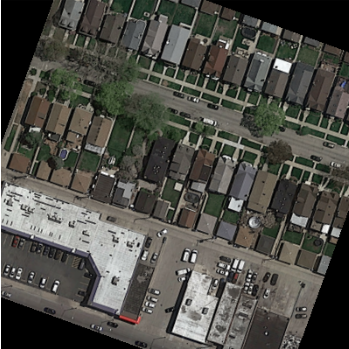
\includegraphics[width=0.35\columnwidth]{img/rot.png}
 \caption{The black part of the picture are ignore during the training steps}
 \vspace{-3mm}
 \label{fig:denoise-fourier}
\end{figure}


\clearpage

\section{Results}
\label{sec:results}
\subsection{your method}
	The CNN was trained for XXX epochs, each consisting of XXX batches of 4 images, on a NVIDIA GeForce GTX graphics card with 2 GB of VRAM. In order to compare different CNNs models we used 4-fold cross validation. Figure XX shows the estimated F1 scores of our main CNN models compared to the aforementioned three baselines and agrees with the F1 score obtained on Kaggle (XXX\%). Even without any preprocessing other than data augmentation our CNN outperformed the baselines and confirmed their superiority in solving this kind of tasks.
\subsection{Unet}
	After 10000 iteration with a learning rate $\lambda = 10^{-3}$ we have obtained a accuracy of 93.35\% on the validation set where the labels are unkown.
	\begin{figure}[h]
		\centering
		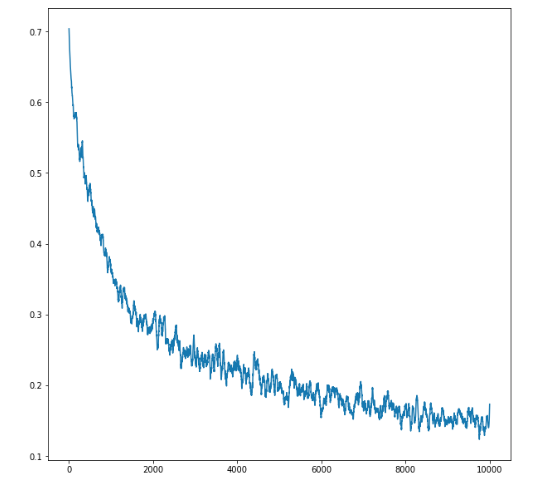
\includegraphics[width=0.8\columnwidth]{img/loss_unet.png}
		\caption{Evolution of the training accuracy regarding the number of iteration}
		\label{fig:lossunet}
	\end{figure}
\subsection{Precision and recall analysis}

	\begin{figure}[h]
		\centering
		$\vcenter{\hbox{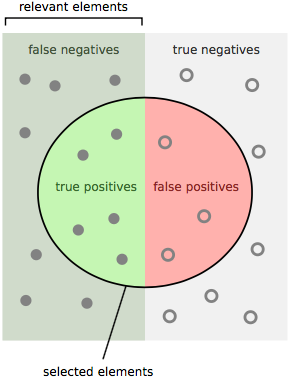
\includegraphics[width=0.25\columnwidth]{img/pr_explain1.png}}}$
		$\vcenter{\hbox{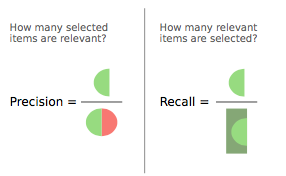
\includegraphics[width=0.6\columnwidth]{img/pr_explain2.png}}}$

		\label{fig:pr_explain}
	\end{figure}

	To compare our result we are using the Precision Recall method (PR). It's focusing on the relevance of the prediction and the labels of a test set. To compute the PR values we split the initial dataset into a training set and a test set where we know the ground thruths.

	Then after the training we can compare our predictions with the ground thruth of the test set. We gradually increase the threshold that set the limit of the probability of the background and the road segment's pixels to compute different PR values on all the test set in order to plot the following graph.

	\begin{figure}[h]
		\centering
		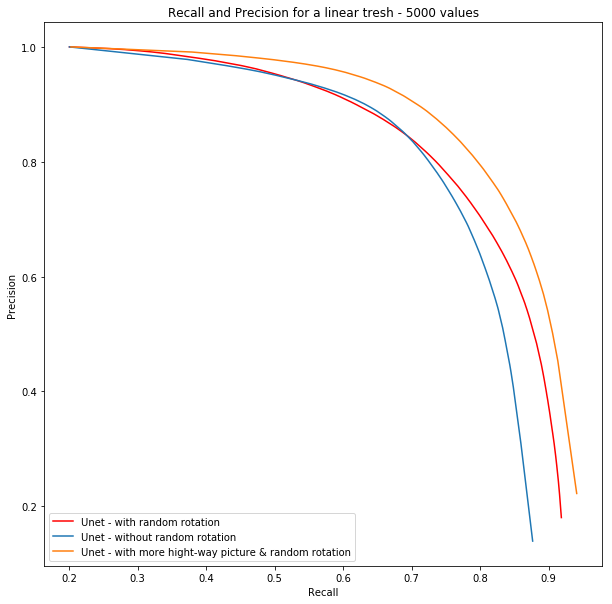
\includegraphics[width=0.8\columnwidth]{img/pr_curve.png}
		\caption{Precision and recall evolution regarding our different methods}
		\label{fig:pr}
	\end{figure}

	With UNet we can see the evolution with the different approaches. The random rotation and the enhancement of the outlayer are actually improving our results our validation set.

\section{Conclusion}
\label{sec:conclusion}
The model we designed proved to be versatile and effective in predicting correctly. However, our model failed in recognizing narrow roads, especially when they were covered by shadows, as show in Figure XX. This problem is due to the fact that those types of roads are almost inexistent in the training set while present in many images of the test set. Moreover, the train and test datasets were mainly restricted to cities. To obtain a model that would efficiently work with a wider range of input images, e.g. images with snow, contry images or on different metheorical conditions, we would require a bigger and diverse training set.


\bibliographystyle{IEEEtran}
\bibliography{groupRoadSegmentationFault-literature}

\end{document}
